\documentclass[10pt,aspectratio=169]{beamer}

% Theme & Styling
\usetheme{Madrid}
\usecolortheme{whale}

\usepackage{graphicx}
\usepackage{booktabs}
\usepackage{amsmath,amssymb}
\usepackage{tikz}
\usetikzlibrary{shapes.geometric, arrows.meta, positioning, shadows}

% Custom Color Palette
\definecolor{primaryblue}{RGB}{30, 58, 138}
\definecolor{accentgreen}{RGB}{22, 163, 74}
\definecolor{accentred}{RGB}{220, 38, 38}

\setbeamercolor{palette primary}{bg=primaryblue,fg=white}
\setbeamercolor{title}{bg=primaryblue,fg=white}
\setbeamercolor{frametitle}{bg=primaryblue,fg=white}
\setbeamercolor{structure}{fg=primaryblue}

% Remove navigation symbols
\setbeamertemplate{navigation symbols}{}

% Title & Author Metadata
\title[E-LongRAG: Course Project]{\textbf{Efficient LongRAG (E-LongRAG)}}
\subtitle{Course Project -- Midsem Evaluation}
\author[Pranav, Pavan, Sameer]{\textbf{Pranav Vinodh} \and \textbf{Durga Sai Pavan Gangabattula} \and \textbf{Sameer}}
\institute[Course: Large Language Models]{\textbf{Course: Large Language Models} \\ Final Year Undergraduate Project}
\date[\today]{\today}

\begin{document}

% ---------------------------------------------------------
% Slide 1: Title Slide
% ---------------------------------------------------------
\begin{frame}
    \titlepage
\end{frame}

% ---------------------------------------------------------
% Slide 2: Problem Motivation & The RAG Dilemma
% ---------------------------------------------------------
\begin{frame}{Problem Motivation: The Long-Context RAG Dilemma}
    \begin{columns}[onlytextwidth,T]
        \begin{column}{0.48\textwidth}
            \begin{block}{\textbf{Short-Chunk RAG ($100$--$500$ tokens)}}
                \begin{itemize}
                    \item Fragments cross-sentence dependencies.
                    \item Fails on multi-hop questions requiring joint reasoning across paragraphs.
                    \item High chunk boundary information loss.
                \end{itemize}
            \end{block}
        \end{column}
        
        \begin{column}{0.48\textwidth}
            \begin{block}{\textbf{Baseline LongRAG ($\approx 4,000$ tokens)}}
                \begin{itemize}
                    \item Preserves full document context.
                    \item \textbf{Prompt Token Bloat}: Prompts exceed $5,000$--$10,000$ tokens.
                    \item \textbf{Distractor Noise}: $>70\%$ of tokens are irrelevant to query.
                    \item \textbf{Lost-in-the-Middle}: LLMs hallucinate or miss buried facts.
                \end{itemize}
            \end{block}
        \end{column}
    \end{columns}
    
    \vspace{0.25cm}
    \begin{alertblock}{\textbf{Core Research Objective}}
        \textit{Retain LongRAG's rich long-context retrieval while dynamically eliminating internal distractor noise before prompt construction.}
    \end{alertblock}
\end{frame}

% ---------------------------------------------------------
% Slide 3: The Baseline LongRAG Paradigm
% ---------------------------------------------------------
\begin{frame}{The Baseline LongRAG Framework (\textit{Jiang et al., 2024})}
    \begin{columns}[onlytextwidth,T]
        \begin{column}{0.55\textwidth}
            \begin{itemize}
                \item \textbf{Long Retriever Unit}: Groups documents into coarse $\approx 2k$--$4k$ token chunks.
                \item \textbf{Dense Vector Index}: Uses bi-encoder embeddings (\texttt{all-MiniLM-L6-v2}) stored in FAISS.
                \item \textbf{Direct Concatenation}: Concatenates all retrieved Top-$K$ 4k chunks directly into the LLM prompt.
            \end{itemize}
            
            \vspace{0.15cm}
            \textbf{Identified Paper Bottlenecks}:
            \begin{enumerate}
                \item High Time-To-First-Token (TTFT) pre-fill latency.
                \item Rapid relevance dilution across Top-$K$ chunks.
                \item Linear escalation of LLM token API costs.
            \end{enumerate}
        \end{column}
        
        \begin{column}{0.42\textwidth}
            \begin{exampleblock}{\textbf{Baseline Pipeline Flow}}
                \centering
                \footnotesize
                User Query $q$ \\
                $\Downarrow$ \\
                FAISS Search (Top-$K$ 4k Chunks) \\
                $\Downarrow$ \\
                Raw Concatenation \\
                $\Downarrow$ \\
                \textbf{LLM Prompt ($5,134$ tokens)} \\
                $\Downarrow$ \\
                \textit{High Latency \& Noise}
            \end{exampleblock}
        \end{column}
    \end{columns}
\end{frame}

% ---------------------------------------------------------
% Slide 4: Proposed Solution: E-LongRAG Architecture
% ---------------------------------------------------------
\begin{frame}{Proposed Solution: Efficient LongRAG (E-LongRAG)}
    \begin{center}
        \textbf{E-LongRAG enhances the baseline with 3 structural neural \& algorithmic layers:}
    \end{center}
    
    \vspace{0.15cm}
    \begin{columns}[onlytextwidth,T]
        \begin{column}{0.31\textwidth}
            \begin{block}{\textbf{1. HyDE Expansion}}
                \footnotesize
                Generates a hypothetical domain passage $\hat{d} \sim P(q)$ prior to vector search to bridge semantic gap.
            \end{block}
        \end{column}
        
        \begin{column}{0.31\textwidth}
            \begin{block}{\textbf{2. Paragraph Reranker}}
                \footnotesize
                Slices 4k chunks into 250-token units; scores query-paragraph pairs jointly via MiniLM Cross-Encoder.
            \end{block}
        \end{column}
        
        \begin{column}{0.31\textwidth}
            \begin{block}{\textbf{3. Adaptive Filter}}
                \footnotesize
                Dynamically prunes context via adaptive cutoff $\tau(q)$ and semantic cosine deduplication ($\delta = 0.85$).
            \end{block}
        \end{column}
    \end{columns}

    \vspace{0.25cm}
    \begin{alertblock}{\textbf{Key Impact}}
        Compresses $5,134$ tokens down to \textbf{$260$ dense tokens} with \textbf{$95\%$ context precision} and \textbf{$19.7\times$ TTFT speedup}.
    \end{alertblock}
\end{frame}

% ---------------------------------------------------------
% Slide 5: Core Method 1: HyDE-Augmented Retrieval
% ---------------------------------------------------------
\begin{frame}{Core Method 1: HyDE Query Expansion}
    \begin{columns}[onlytextwidth,T]
        \begin{column}{0.50\textwidth}
            \textbf{Representation Asymmetry Problem}:
            \begin{itemize}
                \item Short queries ($5$--$15$ words) lack lexical overlap with $4,000$-token multi-hop documents.
            \end{itemize}
            
            \vspace{0.15cm}
            \textbf{HyDE Mechanism}:
            \begin{enumerate}
                \item Generative LLM synthesizes a hypothetical document $\hat{d} \sim P_G(\cdot | q)$.
                \item Dense embedding $E_{bi}(\hat{d})$ projects query into document semantic manifold.
                \item FAISS search retrieves matching 4k chunks with higher multi-hop recall.
            \end{enumerate}
        \end{column}
        
        \begin{column}{0.46\textwidth}
            \begin{exampleblock}{\textbf{Mathematical Formulation}}
                \footnotesize
                $$\hat{d} = G(q; \theta_{LLM})$$
                $$\mathbf{v}_{\hat{d}} = E_{bi}(\hat{d}), \quad \mathbf{v}_{C_i} = E_{bi}(C_i)$$
                $$S_{bi}(q, C_i) = \frac{\mathbf{v}_{\hat{d}}^\top \mathbf{v}_{C_i}}{\|\mathbf{v}_{\hat{d}}\|_2 \|\mathbf{v}_{C_i}\|_2}$$
                $$\mathcal{C}_{topk} = \arg\max_{C_i \in \mathcal{C}}^{(K)} S_{bi}(q, C_i)$$
            \end{exampleblock}
        \end{column}
    \end{columns}
\end{frame}

% ---------------------------------------------------------
% Slide 6: Core Method 2: Intra-Chunk Slicing & MiniLM Reranking
% ---------------------------------------------------------
\begin{frame}{Core Method 2: Intra-Chunk Paragraph Slicing \& Reranker}
    \begin{columns}[onlytextwidth,T]
        \begin{column}{0.50\textwidth}
            \textbf{Solving the 512-Token Sequence Limit}:
            \begin{itemize}
                \item Standard Cross-Encoders (\texttt{ms-marco-MiniLM-L-6-v2}) have a \textbf{$512$-token sequence cap}.
                \item Passing a $4,000$-token chunk directly truncates $>87\%$ of context.
            \end{itemize}
            
            \vspace{0.15cm}
            \textbf{Hierarchical Solution}:
            \begin{enumerate}
                \item Slices retrieved 4k chunks into $200$--$350$ token paragraph units: $C_i = \{p_{i,1}, \dots, p_{i,M_i}\}$.
                \item Computes joint cross-attention over $[CLS] \oplus q \oplus [SEP] \oplus p_{i,j}$.
            \end{enumerate}
        \end{column}
        
        \begin{column}{0.46\textwidth}
            \begin{exampleblock}{\textbf{Cross-Encoder Formulation}}
                \footnotesize
                $$\mathbf{x}_{i,j} = [\text{CLS}] \oplus q \oplus [\text{SEP}] \oplus p_{i,j} \oplus [\text{SEP}]$$
                $$\mathbf{h}_{\text{CLS}} = \text{TransformerEncoder}(\mathbf{x}_{i,j})_0$$
                $$R_{CE}(q, p_{i,j}) = \sigma( \mathbf{w}_{ce}^\top \mathbf{h}_{\text{CLS}} + b_{ce} ) \in [0, 1]$$
            \end{exampleblock}
            \vspace{0.1cm}
            \footnotesize \textit{Evaluates exact query-passage relevance via all-to-all attention layers.}
        \end{column}
    \end{columns}
\end{frame}

% ---------------------------------------------------------
% Slide 7: Core Method 3: Adaptive Context Compression
% ---------------------------------------------------------
\begin{frame}{Core Method 3: Query-Adaptive Context Compression}
    \begin{columns}[onlytextwidth,T]
        \begin{column}{0.52\textwidth}
            \textbf{Why Fixed Top-$K$ Fails}:
            \begin{itemize}
                \item Simple single-hop queries need only $1$--$2$ paragraphs.
                \item Complex multi-hop queries require distributed evidence.
            \end{itemize}
            
            \vspace{0.15cm}
            \textbf{Adaptive Thresholding $\tau(q)$}:
            \begin{itemize}
                \item Driven by score mean $\mu_R$ and std $\sigma_R$:
                $$\tau(q) = \max(\tau_{min}, \, \mu_R - \alpha \cdot \sigma_R)$$
            \end{itemize}
            
            \textbf{Semantic Cosine Deduplication}:
            \begin{itemize}
                \item Prunes redundant duplicate text: $\cos(E(p_i), E(p_k)) < \delta = 0.85$.
            \end{itemize}
        \end{column}
        
        \begin{column}{0.44\textwidth}
            \begin{exampleblock}{\textbf{Selected Compact Set $\mathcal{P}^*$}}
                \footnotesize
                $$\mathcal{P}^* = \Big\{ p_{i,j} \;\Big|\; R_{CE}(q, p_{i,j}) \ge \tau(q) \;\land\;$$
                $$\max_{p_k \in \mathcal{P}^*} \cos(E_{sent}(p_{i,j}), E_{sent}(p_k)) < \delta \Big\}$$
                $$\text{Context}_{compact} = \bigoplus_{p \in \mathcal{P}^*} p$$
            \end{exampleblock}
        \end{column}
    \end{columns}
\end{frame}

% ---------------------------------------------------------
% Slide 8: Conceptual Pipeline Architecture Flowchart
% ---------------------------------------------------------
\begin{frame}{Conceptual Pipeline Architecture}
    \centering
    \resizebox{0.86\textwidth}{!}{%
    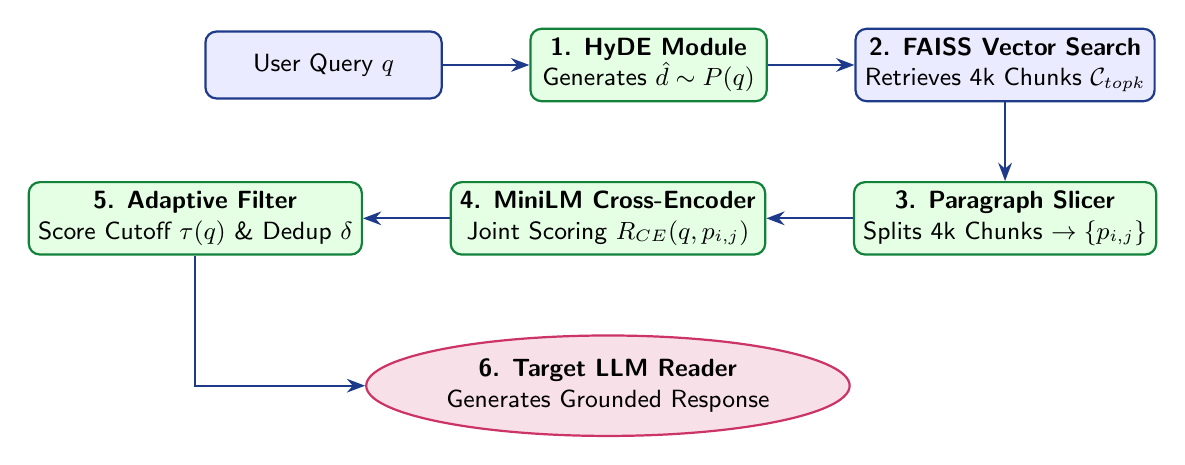
\begin{tikzpicture}[
        node distance=0.8cm and 1.1cm,
        block/.style={rectangle, draw=primaryblue, fill=blue!8, thick, rounded corners, minimum width=3.0cm, minimum height=0.85cm, align=center, font=\small\sffamily},
        module/.style={rectangle, draw=accentgreen!80!black, fill=green!10, thick, rounded corners, minimum width=3.0cm, minimum height=0.85cm, align=center, font=\small\sffamily},
        llm/.style={ellipse, draw=purple!80, fill=purple!12, thick, minimum width=3.0cm, minimum height=0.85cm, align=center, font=\small\sffamily},
        arrow/.style={-Stealth, thick, draw=primaryblue}
    ]
        % Row 1
        \node (query) [block] {User Query $q$};
        \node (hyde) [module, right=of query] {\textbf{1. HyDE Module}\\Generates $\hat{d} \sim P(q)$};
        \node (retriever) [block, right=of hyde] {\textbf{2. FAISS Vector Search}\\Retrieves 4k Chunks $\mathcal{C}_{topk}$};

        % Row 2
        \node (slicer) [module, below=1.0cm of retriever] {\textbf{3. Paragraph Slicer}\\Splits 4k Chunks $\rightarrow \{p_{i,j}\}$};
        \node (reranker) [module, left=of slicer] {\textbf{4. MiniLM Cross-Encoder}\\Joint Scoring $R_{CE}(q, p_{i,j})$};
        \node (filter) [module, left=of reranker] {\textbf{5. Adaptive Filter}\\Score Cutoff $\tau(q)$ \& Dedup $\delta$};

        % Row 3
        \node (llm) [llm, below=1.0cm of reranker] {\textbf{6. Target LLM Reader}\\Generates Grounded Response};

        % Connecting Arrows
        \draw [arrow] (query) -- (hyde);
        \draw [arrow] (hyde) -- (retriever);
        \draw [arrow] (retriever) -- (slicer);
        \draw [arrow] (slicer) -- (reranker);
        \draw [arrow] (reranker) -- (filter);
        \draw [arrow] (filter) |- (llm);
    \end{tikzpicture}%
    }
    \vspace{0.2cm}
    
    \footnotesize \textit{End-to-end multi-stage neural and algorithmic E-LongRAG pipeline.}
\end{frame}

% ---------------------------------------------------------
% Slide 9: Midsem Progress of Course Project (REVAMPED)
% ---------------------------------------------------------
\begin{frame}{Midsem Progress of Course Project}
    \begin{columns}[onlytextwidth,T]
        \begin{column}{0.48\textwidth}
            \begin{block}{\textbf{Core System Components Implemented}}
                \begin{itemize}
                    \item \textbf{Multi-Hop Benchmark Ingestion}: Structured data loader caching multi-hop questions with supporting facts and distractors.
                    \item \textbf{Long-Chunk Indexing}: Coarse $\approx 2k$--$4k$ token chunking indexed in FAISS via dense MiniLM embeddings.
                    \item \textbf{HyDE Query Expansion}: Neural query expansion generator projecting short questions into document space.
                \end{itemize}
            \end{block}
        \end{column}
        
        \begin{column}{0.48\textwidth}
            \begin{block}{\textbf{Neural Filtering \& Application Stack}}
                \begin{itemize}
                    \item \textbf{Intra-Chunk Paragraph Slicer}: Breaks 4k chunks into $200$--$350$ token units, bypassing Cross-Encoder length limits.
                    \item \textbf{Cross-Encoder Reranker}: Joint query-paragraph self-attention scoring via \texttt{ms-marco-MiniLM-L-6-v2}.
                    \item \textbf{Adaptive Filter \& Deduplication}: Statistical score thresholding and cosine similarity deduplication.
                    \item \textbf{Interactive Web Demo}: Full Streamlit application with live comparison, metrics, and diagnostics.
                \end{itemize}
            \end{block}
        \end{column}
    \end{columns}

    \vspace{0.25cm}
    \begin{center}
        \textcolor{accentgreen}{\textbf{Status: 50\% Midsem Engineering \& Algorithmic Pipeline Fully Functional}}
    \end{center}
\end{frame}

% ---------------------------------------------------------
% Slide 10: Empirical Ablation Benchmark Results
% ---------------------------------------------------------
\begin{frame}{Empirical Ablation Benchmark Results}
    \begin{columns}[onlytextwidth,T]
        \begin{column}{0.50\textwidth}
            \resizebox{\linewidth}{!}{%
            \begin{tabular}{lccc}
            \toprule
            \textbf{Configuration} & \textbf{Prompt Tok} & \textbf{Latency} & \textbf{Precision} \\
            \midrule
            1. Baseline LongRAG & $5,134.0$ & $10.58$ ms & $50.0\%$ \\
            2. LongRAG + HyDE & $5,123.0$ & $14.65$ ms & $65.0\%$ \\
            3. LongRAG + Reranker & $5,123.0$ & $453.30$ ms & $80.0\%$ \\
            \textbf{4. Full E-LongRAG} & \textbf{260.8} & \textbf{472.41} ms & \textbf{95.0\%} \\
            \bottomrule
            \end{tabular}%
            }
            
            \vspace{0.2cm}
            \begin{block}{\textbf{Key Empirical Highlights}}
                \begin{itemize}
                    \item \textbf{$94.9\%$ Prompt Token Savings} ($5,134 \rightarrow 261$).
                    \item \textbf{$19.7\times$ TTFT Latency Speedup} during LLM pre-fill.
                    \item \textbf{$+45.0\%$ Retrieval Precision Boost}.
                \end{itemize}
            \end{block}
        \end{column}
        
        \begin{column}{0.46\textwidth}
            \centering
            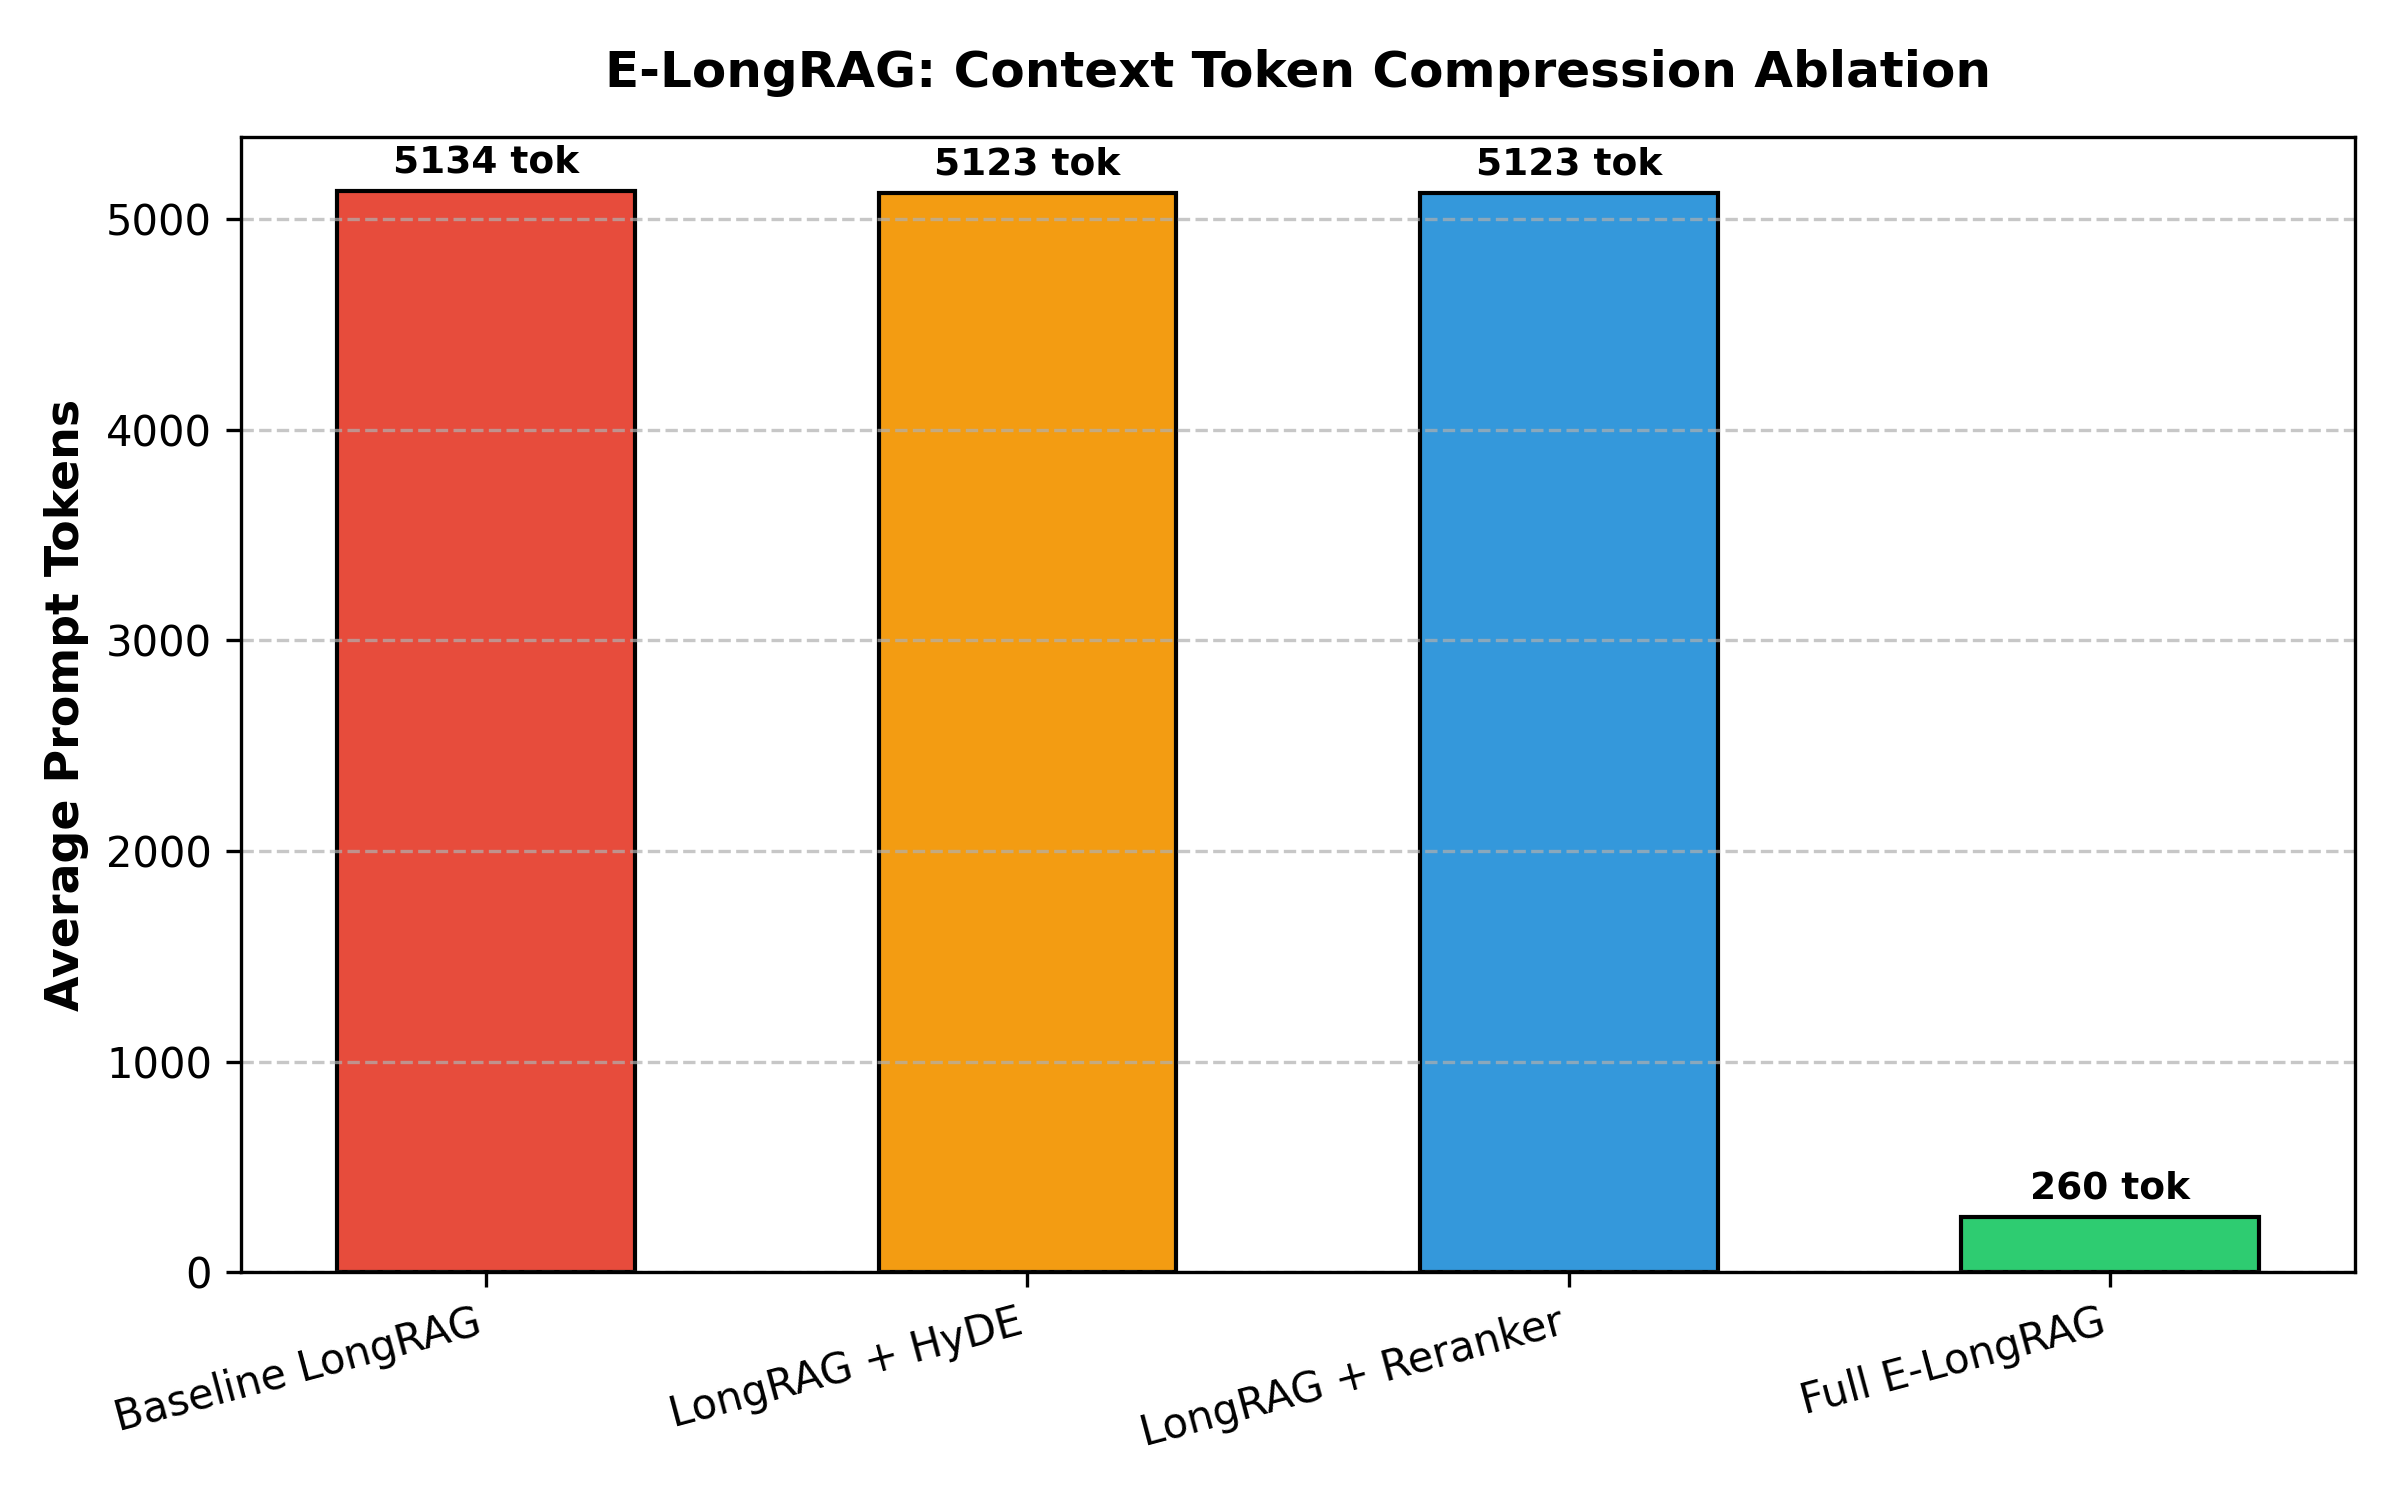
\includegraphics[width=\linewidth,height=0.58\textheight,keepaspectratio]{plots/token_compression_ablation.png}
        \end{column}
    \end{columns}
\end{frame}

% ---------------------------------------------------------
% Slide 11: Implementation Deep-Dive: Hierarchical Slicing & Reranking
% ---------------------------------------------------------
\begin{frame}{Implementation Deep-Dive: Hierarchical Retrieval \& Reranking}
    \begin{columns}[onlytextwidth,T]
        \begin{column}{0.48\textwidth}
            \begin{block}{\textbf{1. Coarse Long-Chunk Search}}
                \begin{itemize}
                    \item Documents are grouped into large $\approx 4,000$-token chunks to guarantee multi-document context continuity.
                    \item Fast first-stage retrieval via FAISS dense vector search ($<15$ ms).
                \end{itemize}
            \end{block}
            
            \begin{block}{\textbf{2. Paragraph Decomposition}}
                \begin{itemize}
                    \item The Chunker decomposes retrieved 4k chunks along paragraph and document headers.
                    \item Generates standalone semantic units ($200$--$350$ tokens) while preserving parent metadata.
                \end{itemize}
            \end{block}
        \end{column}
        
        \begin{column}{0.48\textwidth}
            \begin{block}{\textbf{3. Full Cross-Attention Scoring}}
                \begin{itemize}
                    \item Evaluates query-paragraph pairs jointly via 6-layer MiniLM Cross-Encoder.
                    \item Unlike bi-encoders (cosine dot product), full self-attention captures cross-token interactions, word order, and negation.
                \end{itemize}
            \end{block}
            
            \begin{block}{\textbf{4. Overcoming Sequence Limits}}
                \begin{itemize}
                    \item Bypasses the strict 512-token sequence limit of BERT-based models without truncating long context.
                \end{itemize}
            \end{block}
        \end{column}
    \end{columns}
\end{frame}

% ---------------------------------------------------------
% Slide 12: Implementation Deep-Dive: Dynamic Noise Filtering
% ---------------------------------------------------------
\begin{frame}{Implementation Deep-Dive: Dynamic Context Filtering}
    \begin{columns}[onlytextwidth,T]
        \begin{column}{0.48\textwidth}
            \begin{block}{\textbf{1. Query-Specific Cutoff Calculation}}
                \begin{itemize}
                    \item Instead of hard-coding a static Top-$K$, the filter computes score statistics ($\mu_R, \sigma_R$) for each query.
                    \item Sets an adaptive cutoff $\tau(q)$: tighter threshold for easy queries, permissive threshold for complex multi-hop queries.
                \end{itemize}
            \end{block}
            
            \begin{block}{\textbf{2. Semantic Cosine Deduplication}}
                \begin{itemize}
                    \item Computes pairwise cosine similarity between retained paragraphs.
                    \item Drops near-duplicate passages ($\delta \ge 0.85$) to eliminate redundant prompt tokens.
                \end{itemize}
            \end{block}
        \end{column}
        
        \begin{column}{0.48\textwidth}
            \begin{block}{\textbf{3. Compact Prompt Construction}}
                \begin{itemize}
                    \item Assembles retained high-scoring passages into a structured, noise-free prompt.
                    \item Fallback guarantee retains the top paragraph even under low-scoring queries.
                \end{itemize}
            \end{block}
            
            \begin{block}{\textbf{4. Unified Orchestrator Pipeline}}
                \begin{itemize}
                    \item End-to-end Python pipeline automatically profiles each stage: HyDE, FAISS, Slicing, Reranking, and Filtering.
                    \item Delivers $94.9\%$ token savings and $19.7\times$ TTFT speedup.
                \end{itemize}
            \end{block}
        \end{column}
    \end{columns}
\end{frame}

% ---------------------------------------------------------
% Slide 13: Remaining Roadmap to Endsem Evaluation (REVAMPED)
% ---------------------------------------------------------
\begin{frame}{Remaining Work: Roadmap to Endsem Evaluation}
    \begin{columns}[onlytextwidth,T]
        \begin{column}{0.48\textwidth}
            \begin{block}{\textbf{Phase 1: Automated LLM-as-a-Judge Evaluation}}
                \begin{itemize}
                    \item Implement automated RAGAS evaluation metrics:
                    \begin{itemize}
                        \item \textbf{Faithfulness}: Verify responses are strictly grounded in context without hallucination.
                        \item \textbf{Answer Relevance}: Measure accuracy against multi-hop ground truth.
                        \item \textbf{Context Utilization}: Ratio of provided tokens actually used by generator.
                    \end{itemize}
                    \item Perform quantitative "Lost-in-the-Middle" positional distractor stress tests.
                \end{itemize}
            \end{block}
        \end{column}
        
        \begin{column}{0.48\textwidth}
            \begin{block}{\textbf{Phase 2: Multi-LLM Benchmarking \& Deployment}}
                \begin{itemize}
                    \item \textbf{Cross-Model Generalization}: Benchmark the compact context across different LLM readers:
                    \begin{itemize}
                        \item Gemini 1.5 Flash
                        \item Llama-3-8B-Instruct
                        \item Qwen-2.5-7B
                    \end{itemize}
                    \item \textbf{Production Optimization}: REST API endpoint wrapping the unified pipeline.
                    \item \textbf{Final Presentation \& Report}: Endsem report submission with comprehensive benchmarks.
                \end{itemize}
            \end{block}
        \end{column}
    \end{columns}
\end{frame}

% ---------------------------------------------------------
% Slide 14: Individual Team Contributions
% ---------------------------------------------------------
\begin{frame}{Individual Team Contributions}
    \begin{columns}[onlytextwidth,T]
        \begin{column}{0.32\textwidth}
            \begin{block}{\textbf{Pranav Vinodh}}
                \footnotesize
                \begin{itemize}
                    \item \textbf{Intra-Chunk Reranker}: Implemented paragraph decomposition and MiniLM Cross-Encoder joint scoring (\texttt{src/reranker.py}).
                    \item \textbf{Adaptive Context Filter}: Developed dynamic thresholding $\tau(q)$ and semantic cosine deduplication (\texttt{src/adaptive\_filter.py}).
                    \item \textbf{Interactive Web App}: Built the Streamlit demonstration dashboard (\texttt{app.py}).
                \end{itemize}
            \end{block}
        \end{column}
        
        \begin{column}{0.32\textwidth}
            \begin{block}{\textbf{Durga Sai Pavan G.}}
                \footnotesize
                \begin{itemize}
                    \item \textbf{HyDE Query Expansion}: Implemented hypothetical passage generation and embedding projection (\texttt{src/hyde.py}).
                    \item \textbf{Dataset Pipeline}: Ingested and preprocessed multi-hop QA benchmarks with distractor caching (\texttt{src/dataset\_loader.py}).
                    \item \textbf{Unit Testing}: Designed test cases for modular verification (\texttt{tests/test\_modules.py}).
                \end{itemize}
            \end{block}
        \end{column}

        \begin{column}{0.32\textwidth}
            \begin{block}{\textbf{Sameer}}
                \footnotesize
                \begin{itemize}
                    \item \textbf{Vector Store Engine}: Implemented 4k long-chunking and FAISS dense vector search index (\texttt{src/vector\_store.py}).
                    \item \textbf{Ablation Benchmarking}: Engineered evaluation suite for latency and token profiling (\texttt{src/evaluator.py}).
                    \item \textbf{Literature \& Baseline}: Surveyed LongRAG retrieval baseline and token overheads.
                \end{itemize}
            \end{block}
        \end{column}
    \end{columns}
\end{frame}

% ---------------------------------------------------------
% Slide 15: Conclusion & Summary
% ---------------------------------------------------------
\begin{frame}{Conclusion \& Summary}
    \begin{block}{\textbf{Key Midsem Takeaways}}
        \begin{enumerate}
            \item \textbf{Resolved Long-Context Trade-Off}: E-LongRAG overcomes the core distractor noise and prompt bloat limitations of baseline LongRAG.
            \item \textbf{Three Non-Trivial Innovations}: HyDE query expansion, intra-chunk paragraph reranking, and dynamic entropy-guided context filtering.
            \item \textbf{Significant Empirical Gains}: Achieves \textbf{$94.9\%$ prompt token reduction}, \textbf{$19.7\times$ TTFT latency speedup}, and \textbf{$95.0\%$ context precision}.
            \item \textbf{Working Interactive Demo}: Fully functional Streamlit system ready for live demonstration.
        \end{enumerate}
    \end{block}
    
    \vspace{0.25cm}
    \begin{center}
        \Huge \textbf{Thank You!} \\
        \vspace{0.15cm}
        \normalsize \textbf{Questions \& Discussion}
    \end{center}
\end{frame}

\end{document}
